%-- Add sections and your outline will be created automatically --%
\subsection{Lid-driven cavity}

% Frame starts a new slide
\begin{frame}
    \frametitle{Lid-driven cavity}
\begin{itemize}
\item Simple test case often used for verification and validation
\item Re = 1000
\end{itemize}
\begin{figure}
\centering
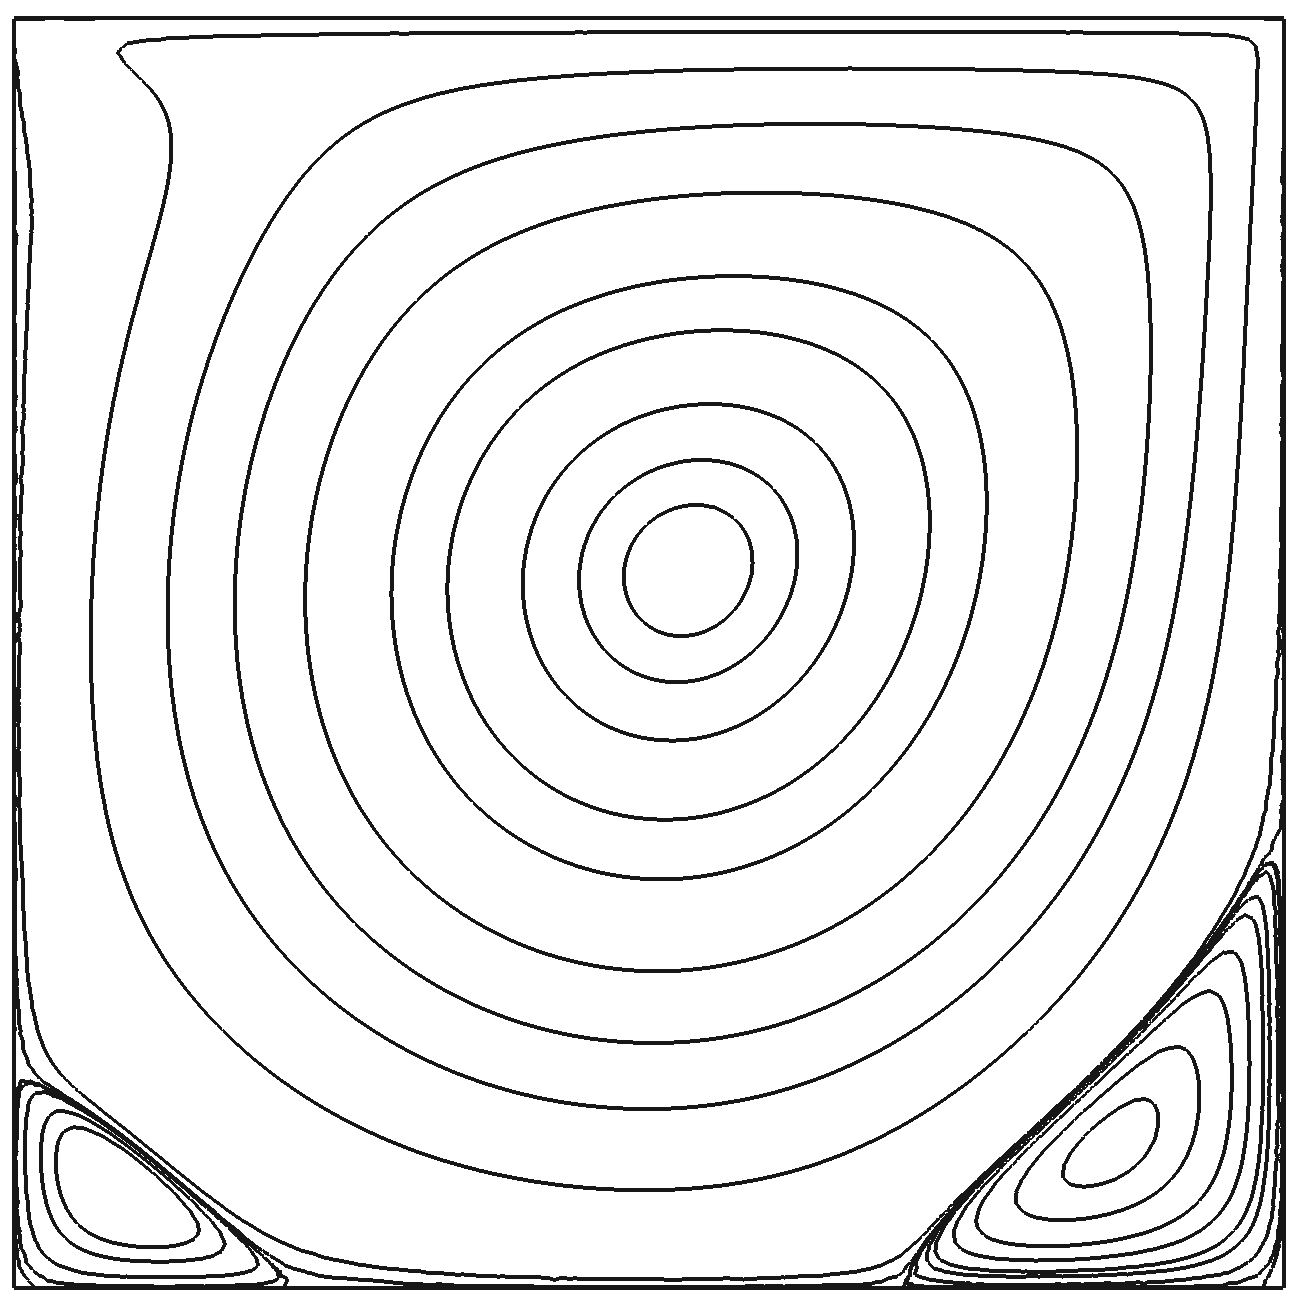
\includegraphics[width=0.4\textwidth]{./driven_cavity/driven_cavity_streamfunction.png}
\caption{Streamfunction contours in converged solution for $h=1/128$.}
\end{figure}
% end my slide
\end{frame}

\begin{frame}
    \frametitle{Lid-driven cavity}
\begin{figure}
\centering
\subfigure[vorticity contours in converged solution for \mbox{$h=1/128$}]{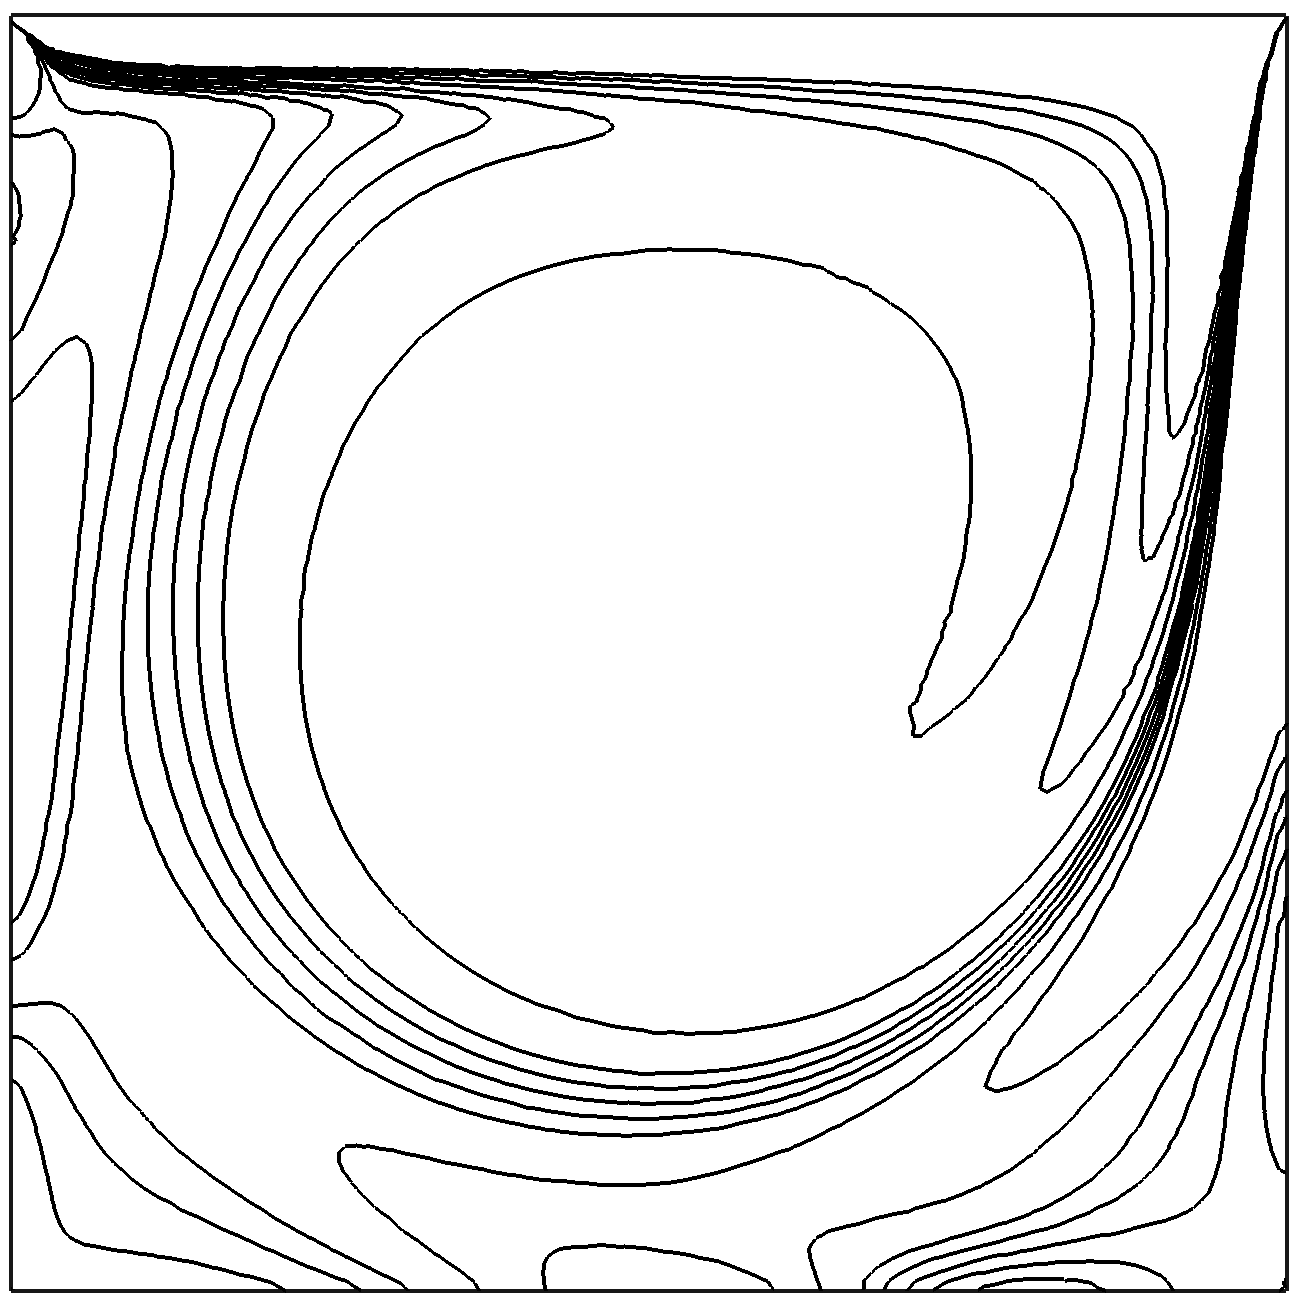
\includegraphics[width=0.35\textwidth]{./driven_cavity/driven_cavity_vorticity.png}}
\hspace{10mm}
\subfigure[error vs. experiment]{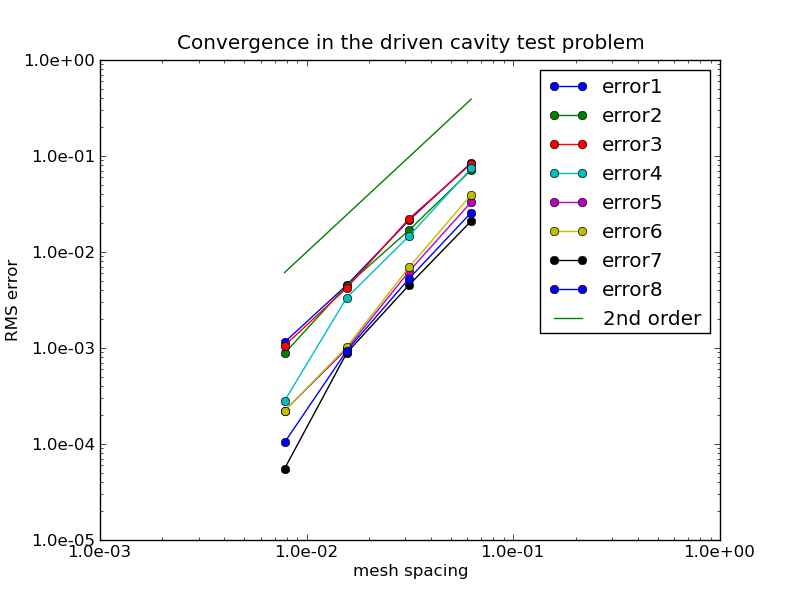
\includegraphics[width=0.45\textwidth]{./driven_cavity/driven_cavity_error_plot.png}}
\caption{The error metrics are listed in the manual.}
\end{figure}
\end{frame}




